\documentclass[11pt]{article}

% ==== Paquetes ====
\usepackage[utf8]{inputenc}
\usepackage[T1]{fontenc}
\usepackage[spanish]{babel}
\usepackage{amsmath, amssymb, amsfonts}
\usepackage{graphicx}
\usepackage{caption}
\usepackage{subcaption}
\usepackage{float}
\usepackage{geometry}
\usepackage{hyperref}
\usepackage{minted}
\usepackage{mdframed}
\geometry{margin=2.3cm}

\usemintedstyle{friendly}
\setminted{fontsize=\scriptsize, breaklines=true}

% ==== Metadatos ====
\title{IEE3682 - Electro-óptica \\ Tarea 5}
\author{Nicolás Seguel}
\date{Noviembre 2025}

\begin{document}
\maketitle

% ================= PROBLEMA 1 =================
\section*{Problema 1 (10 puntos)}

Un haz de luz colimado con polarización lineal orientada $45^\circ$ respecto a la vertical, de 
$\lambda = 640$ nm, se propaga por el aire horizontalmente, incidiendo en una ventana de cuarzo 
de 6 mm de espesor orientada en $45^\circ$ en el plano horizontal. El haz de luz se refleja parcialmente 
en cada interfaz de la ventana, resultando en múltiples transmisiones y reflexiones parciales de la luz.

\begin{enumerate}
    \item[(a)] Calcule la potencia en la primera transmisión.
    \item[(b)] Calcule la potencia en la primera y en la segunda reflexión.
    \item[(c)] Calcule la separación lateral entre la primera y segunda reflexión.
\end{enumerate}

\subsection*{Solución (a)}

Asumiendo un índice de refracción del cuarzo $n = 1.46$, y usando las fórmulas de Fresnel para la reflexión y transmisión con polarización lineal, tenemos:

\begin{align*}
    r_x &= \frac{n_1 \cos(\theta_1) - n_2 \cos(\theta_2)}{n_1 \cos(\theta_1) + n_2 \cos(\theta_2)}, \quad t_x = 1 + r_x \\
    r_y &= \frac{n_1 \sec(\theta_1) - n_2 \sec(\theta_2)}{n_1 \sec(\theta_1) + n_2 \sec(\theta_2)}, \quad t_y = (1 + r_y) \frac{\cos(\theta_1)}{\cos(\theta_2)}
\end{align*}

Calculamos los ángulos de incidencia y transmisión:

\begin{align*}
    \theta_1 &= 45^\circ \\
    \theta_2 &= \arcsin\left(\frac{n_1}{n_2} \sin(\theta_1)\right) = \arcsin\left(\frac{1}{1.46} \sin(45^\circ)\right) \approx 28.97^\circ
\end{align*}

Calculamos los coeficientes de reflexión y transmisión:

\begin{align*}
    r_x &\approx \frac{1 \cdot \cos(45^\circ) - 1.46 \cdot \cos(28.97^\circ)}{1 \cdot \cos(45^\circ) + 1.46 \cdot \cos(28.97^\circ)} \approx -0.287 \\
    t_x &\approx 1 + r_x \approx 0.712 \\
    r_y &\approx \frac{1 \cdot \sec(45^\circ) - 1.46 \cdot \sec(28.97^\circ)}{1 \cdot \sec(45^\circ) + 1.46 \cdot \sec(28.97^\circ)} \approx -0.0825 \\
    t_y &\approx (1 + r_y) \frac{\cos(45^\circ)}{\cos(28.97^\circ)} \approx 0.7415
\end{align*}

Asumiendo que la potencia inicial es 1, la potencia en la primera reflexión es:

\begin{align*}
    \mathcal{R}  &= \left(\frac{|r_x|^2 + |r_y|^2}{2}\right) \\
    &\approx \left(\frac{(-0.287)^2 + (-0.0825)^2}{2}\right) \\
    &\approx \left(\frac{0.0824 + 0.0068}{2}\right) \\
    &\approx \cdot 0.0446
\end{align*}

Por lo que la potencia transmitida dentro del cuarzo es:

\begin{align*}
    \mathcal{T}  &= 1 - \mathcal{R}  \\
    &\approx 1 - 0.0446 \\
    &\approx 0.9554
\end{align*}

Ahora calculamos la potencia en la primera transmisión a través de la segunda interfaz:

\begin{align*}
    r_x' = \frac{1.46 \cdot \cos(28.97^\circ) - 1 \cdot \cos(45^\circ)}{1.46 \cdot \cos(28.97^\circ) + 1 \cdot \cos(45^\circ)} \approx 0.0825 \\
    r_y' = \frac{1.46 \cdot \sec(28.97^\circ) - 1 \cdot \sec(45^\circ)}{1.46 \cdot \sec(28.97^\circ) + 1 \cdot \sec(45^\circ)} \approx 0.287 \\
\end{align*}

La potencia reflejada en la segunda interfaz es:

\begin{align*}
    \mathcal{R}' &= \left(\frac{|r_x'|^2 + |r_y'|^2}{2}\right) \\
    &\approx \left(\frac{(0.0825)^2 + (0.287)^2}{2}\right) \\
    &\approx \left(\frac{0.0068 + 0.0824}{2}\right) \\
    &\approx 0.0446
\end{align*}

Por lo que la potencia transmitida a través de la segunda interfaz es:

\begin{align*}
    \mathcal{T}' &= 1 - \mathcal{R}' \\
    &\approx 1 - 0.0446 \\
    &\approx 0.9554
\end{align*}

Finalmente, la potencia en la primera transmisión es:

\begin{align*}
    P_{\text{transmitida}} &= \mathcal{T} \cdot \mathcal{T}' \\
    &\approx 0.9554 \cdot 0.9554 \\
    &\approx 0.9128
\end{align*}

\subsection*{Solución (b)}

La potencia en la primera reflexión ya fue calculada como:

\begin{align*}
    P_{\text{primera reflexión}} &= \mathcal{R} \\
    &\approx 0.0446
\end{align*}

La potencia en la segunda reflexión se calcula considerando la transmisión a través de la primera interfaz, la reflexión en la segunda interfaz y la transmisión de vuelta a través de la primera interfaz:

\begin{align*}
    P_{\text{segunda reflexión}} &= \mathcal{T} \cdot \mathcal{R}' \cdot \mathcal{T} \\
    &\approx 0.9554 \cdot 0.0446 \cdot 0.9554 \\
    &\approx 0.0407
\end{align*}

\subsection*{Solución (c)}

La separación lateral entre la primera y segunda reflexión se puede calcular usando la geometría del sistema. La distancia entre las reflexiones es:

\begin{align*}
    \Delta x &= 2 d \tan(\theta_2) \\
    &= 2 \cdot 6\ \text{mm} \cdot \tan(28.97^\circ) \\
    &\approx 2 \cdot 6\ \text{mm} \cdot 0.5543 \\
    &\approx 6.64\ \text{mm}
\end{align*}

% ---------------------------------------------------------

\section*{Problema 2 (20 puntos)}

En un microscopio de fluorescencia se adquiere una imagen de una muestra plana con microesferas 
fluorescentes, con tiempo de exposición 1 s. Las microesferas son de 100 nm de diámetro y emiten 
luz de 518 nm. La imagen se registra con una cámara CMOS con fotodiodos de Silicio, con eficiencia 
cuántica 80\% y factor de conversión 0.46 electrones por cada cuenta de intensidad. Cada píxel 
abarca $0.16\times0.16\ \mu\text{m}^2$ de la muestra. Las cuentas de intensidad de los píxeles tienen un 
offset igual a 100, es decir, otra imagen similar en oscuridad total tiene valor promedio 100 en los 
píxeles. Analizando la imagen de microesferas obtenida en el archivo \texttt{img.tif}, estime las siguientes 
cantidades:

\begin{enumerate}
    \item[(a)] Resolución y apertura numérica del microscopio.
    \item[(b)] Número de cuentas de intensidad promedio del fondo de iluminación en la muestra, 
    donde no hay microesferas.
    \item[(c)] Número total de cuentas de intensidad promedio detectadas en una microesfera, 
    por sobre el nivel promedio de fondo.
    \item[(d)] Corriente total generada en la cámara por una microesfera.
    \item[(e)] Potencia óptica incidente en la cámara desde una microesfera.
    \item[(f)] Potencia óptica irradiada por una microesfera, asumiendo que el microscopio 
    captura el ángulo sólido correspondiente a la apertura numérica calculada, y que el 
    sistema óptico hasta la cámara transmite el 90\%.
    \item[(g)] Tiempo de exposición mínimo que permitiría detectar las microesferas con 
    SNR = 2 por sobre el nivel de ruido del fondo.
\end{enumerate}

\begin{figure}[H]
    \centering
    %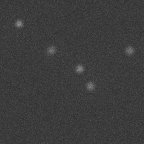
\includegraphics[width=0.6\textwidth]{img.png}
    \caption{Muestra plana de microesferas fluorescentes.}
\end{figure}

\subsection*{Solución (a)}



% ---------------------------------------------------------

\section*{Problema 3 (10 puntos)}

Considere una distribución de $N$ moléculas puntuales localizadas en posiciones $\vec{\rho}_n$, 
cada una emitiendo fluorescencia con intensidades dependientes del tiempo $f_n(t)$. 
Estas se observan mediante un microscopio de campo amplio estándar. 
La intensidad resultante registrada por la cámara es:

\[
I(\vec{\rho}, t) = \sum_{n=1}^{N} \text{PSF}(\vec{\rho} - \vec{\rho}_n)\, f_n(t).
\]

\begin{enumerate}
    \item[(a)] Muestre que, si las intensidades $f_n(t)$ son independientes entre sí, entonces 
    una imagen construida a partir de la varianza temporal en cada posición $\vec{\rho}$ viene dada por:
    \[
    \sigma_I^2(\vec{\rho}) = \sum_{n=1}^{N} \text{PSF}^2(\vec{\rho} - \vec{\rho}_n)\, \sigma_n^2,
    \]
    donde $\sigma_n^2$ es la varianza temporal de $f_n(t)$.Este tipo de imagen es inusual, ya que no representa los niveles medios de fluorescencia, sino las varianzas de dichos niveles. Sin embargo, esto puede conducir a una técnica de superresolución denominada Superresolution Optical Fluctuation Imaging (SOFI), al aprovechar el conocimiento previo de las estadísticas de fluorescencia y el hecho de que PSF2 es más angosta que PSF.

    \item[(b)] Considere moléculas que producen fluorescencia con estadística gaussiana. 
    Reescriba el resultado anterior en términos de los niveles medios de fluorescencia $\langle f_n \rangle$.

    \item[(c)] Compruebe que no se obtiene el mismo resultado al simplemente elevar al cuadrado 
    la imagen inicial, es decir, compare el resultado anterior con $\langle I(\vec{\rho}) \rangle^2$.
\end{enumerate}

\end{document}